\begin{pastexam}[label={px:gw3-102-ds-02}]{關務三等資訊處理 102 年 第二題}
（申論；20 分）

已知一棵二元樹（binary tree）的前序走訪（preorder traversal）與中序走訪（inorder traversal）之結果分別如下：
（每小題 10 分，共 20 分）\\
前序－A B D E G H C F I\\
中序－D B G E H A C I F
\begin{itemize}[leftmargin=2.2em]
\item[㈠] 請繪出這棵二元樹。
\item[㈡] 這棵二元樹的後序走訪（postorder traversal）結果為何？
\end{itemize}
\end{pastexam}

\begin{pastsoln}
答案：㈠ 樹如下圖；㈡ D G H E B I F C A。

\textbf{㈠} 前序加中序重建（資結書第~7.4~節，虛擬碼~7.5）：前序的第一個是根；在中序裡找到根，左邊是左子樹、
右邊是右子樹；左子樹有幾個點，前序在根之後就取幾個給左子樹，其餘給右子樹。 做法和歷屆試題~\ref{px:gk3-098-ds-01}
（中序加後序）相同，只是根改從前序的開頭拿。
\begin{center}
\small
\begin{tabular}{llll}
\toprule
前序 & 中序 & 根 & 左子樹／右子樹（中序） \\
\midrule
A B D E G H C F I & D B G E H A C I F & A & D B G E H ／ C I F \\
B D E G H & D B G E H & B & D ／ G E H \\
E G H & G E H & E & G ／ H \\
C F I & C I F & C & 空 ／ I F \\
F I & I F & F & I ／ 空 \\
\bottomrule
\end{tabular}
\end{center}
第一列：A 在中序裡左邊有 $5$ 個（D B G E H），所以前序 A 之後的 $5$ 個 B D E G H 是左子樹，最後 $3$ 個 C F I
是右子樹。 其餘各列同理（只剩一個點的 D、G、H、I 直接是葉節點）。 得到的樹：
\begin{center}
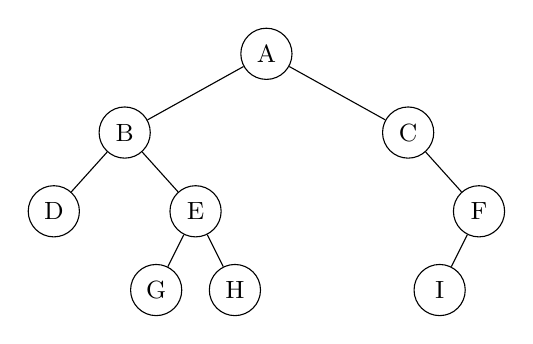
\begin{tikzpicture}[v/.style={circle,draw,minimum size=6.5mm,inner sep=0pt,font=\small},
    level distance=10mm, level 1/.style={sibling distance=36mm},
    level 2/.style={sibling distance=18mm}, level 3/.style={sibling distance=10mm}]
\node[v] {A}
  child {node[v] {B}
    child {node[v] {D}}
    child {node[v] {E} child {node[v] {G}} child {node[v] {H}}}}
  child {node[v] {C}
    child[missing] {}
    child {node[v] {F} child {node[v] {I}} child[missing] {}}};
\end{tikzpicture}
\end{center}
檢查：這棵樹的前序是 A B D E G H C F I、中序是 D B G E H A C I F，都和題目一樣。 前序加中序決定唯一的一棵
二元樹（資結書定理~7.4）。

\textbf{㈡} 後序（左、右、根）：左子樹 B 的部分是 D，接著 E 的子樹 G H E，再 B；右子樹 C 的部分，C 沒有左子樹，
先做 F 的子樹 I F，再 C；最後根 A。 答案 \textbf{D G H E B I F C A}。
\end{pastsoln}
